\documentclass[twoside,11pt]{article}

% ? Specify used packages
\usepackage{graphicx}        %  Use this one for final production.
% \usepackage[draft]{graphicx} %  Use this one for drafting.
% ? End of specify used packages

\pagestyle{myheadings}

% -----------------------------------------------------------------------------
% ? Document identification
% Fixed part
\newcommand{\stardoccategory}  {Starlink User Note}
\newcommand{\stardocinitials}  {SUN}
\newcommand{\stardocsource}    {sun\stardocnumber}
\newcommand{\stardoccopyright}
{Copyright \copyright\ 2010 University of British Columbia and the Science \& Technology Facilities Council}

% Variable part - replace [xxx] as appropriate.
\newcommand{\stardocnumber}    {264.0}
\newcommand{\stardocauthors}   {Andrew G. Gibb \& Tim Jenness}
\newcommand{\stardocdate}      {20 December 2010}
\newcommand{\stardoctitle}     {ORAC-DR --- SCUBA-2 Pipeline Data Reduction}
\newcommand{\stardocversion}   {Version 1.0.0}
\newcommand{\stardocmanual}    {User's Guide}
\newcommand{\stardocabstract}  {

  The ORAC-DR

}
% ? End of document identification
% -----------------------------------------------------------------------------

% +
%  Name:
%     sun258.tex
%
%  Purpose:
%     Documentation for SCUBA-2 data reduction with ORAC-DR
%
%  Authors:
%     AGG: Andy Gibb (UBC)
%
%  History:
%     2010-10-26 (AGG):
%        Initial version
%     {Add further history here}
%
% -

\newcommand{\stardocname}{\stardocinitials /\stardocnumber}
\markboth{\stardocname}{\stardocname}
\setlength{\textwidth}{160mm}
\setlength{\textheight}{230mm}
\setlength{\topmargin}{-2mm}
\setlength{\oddsidemargin}{0mm}
\setlength{\evensidemargin}{0mm}
\setlength{\parindent}{0mm}
\setlength{\parskip}{\medskipamount}
\setlength{\unitlength}{1mm}

% -----------------------------------------------------------------------------
%  Hypertext definitions.
%  ======================
%  These are used by the LaTeX2HTML translator in conjunction with star2html.

%  Comment.sty: version 2.0, 19 June 1992
%  Selectively in/exclude pieces of text.
%
%  Author
%    Victor Eijkhout                                      <eijkhout@cs.utk.edu>
%    Department of Computer Science
%    University Tennessee at Knoxville
%    104 Ayres Hall
%    Knoxville, TN 37996
%    USA

%  Do not remove the %begin{latexonly} and %end{latexonly} lines (used by
%  LaTeX2HTML to signify text it shouldn't process).
%begin{latexonly}
\makeatletter
\def\makeinnocent#1{\catcode`#1=12 }
\def\csarg#1#2{\expandafter#1\csname#2\endcsname}

\def\ThrowAwayComment#1{\begingroup
    \def\CurrentComment{#1}%
    \let\do\makeinnocent \dospecials
    \makeinnocent\^^L% and whatever other special cases
    \endlinechar`\^^M \catcode`\^^M=12 \xComment}
{\catcode`\^^M=12 \endlinechar=-1 %
 \gdef\xComment#1^^M{\def\test{#1}
      \csarg\ifx{PlainEnd\CurrentComment Test}\test
          \let\html@next\endgroup
      \else \csarg\ifx{LaLaEnd\CurrentComment Test}\test
            \edef\html@next{\endgroup\noexpand\end{\CurrentComment}}
      \else \let\html@next\xComment
      \fi \fi \html@next}
}
\makeatother

\def\includecomment
 #1{\expandafter\def\csname#1\endcsname{}%
    \expandafter\def\csname end#1\endcsname{}}
\def\excludecomment
 #1{\expandafter\def\csname#1\endcsname{\ThrowAwayComment{#1}}%
    {\escapechar=-1\relax
     \csarg\xdef{PlainEnd#1Test}{\string\\end#1}%
     \csarg\xdef{LaLaEnd#1Test}{\string\\end\string\{#1\string\}}%
    }}

%  Define environments that ignore their contents.
\excludecomment{comment}
\excludecomment{rawhtml}
\excludecomment{htmlonly}

%  Hypertext commands etc. This is a condensed version of the html.sty
%  file supplied with LaTeX2HTML by: Nikos Drakos <nikos@cbl.leeds.ac.uk> &
%  Jelle van Zeijl <jvzeijl@isou17.estec.esa.nl>. The LaTeX2HTML documentation
%  should be consulted about all commands (and the environments defined above)
%  except \xref and \xlabel which are Starlink specific.

\newcommand{\htmladdnormallinkfoot}[2]{#1\footnote{#2}}
\newcommand{\htmladdnormallink}[2]{#1}
\newcommand{\htmladdimg}[1]{}
\newcommand{\hyperref}[4]{#2\ref{#4}#3}
\newcommand{\htmlref}[2]{#1}
\newcommand{\htmlimage}[1]{}
\newcommand{\htmladdtonavigation}[1]{}

\newenvironment{latexonly}{}{}
\newcommand{\latex}[1]{#1}
\newcommand{\html}[1]{}
\newcommand{\latexhtml}[2]{#1}
\newcommand{\HTMLcode}[2][]{}

%  Starlink cross-references and labels.
\newcommand{\xref}[3]{#1}
\newcommand{\xlabel}[1]{}

%  LaTeX2HTML symbol.
\newcommand{\latextohtml}{\LaTeX2\texttt{HTML}}

%  Define command to re-centre underscore for Latex and leave as normal
%  for HTML (severe problems with \_ in tabbing environments and \_\_
%  generally otherwise).
\renewcommand{\_}{\texttt{\symbol{95}}}

% -----------------------------------------------------------------------------
%  Debugging.
%  =========
%  Remove % on the following to debug links in the HTML version using Latex.

% \newcommand{\hotlink}[2]{\fbox{\begin{tabular}[t]{@{}c@{}}#1\\\hline{\footnotesize #2}\end{tabular}}}
% \renewcommand{\htmladdnormallinkfoot}[2]{\hotlink{#1}{#2}}
% \renewcommand{\htmladdnormallink}[2]{\hotlink{#1}{#2}}
% \renewcommand{\hyperref}[4]{\hotlink{#1}{\S\ref{#4}}}
% \renewcommand{\htmlref}[2]{\hotlink{#1}{\S\ref{#2}}}
% \renewcommand{\xref}[3]{\hotlink{#1}{#2 -- #3}}
%end{latexonly}
% -----------------------------------------------------------------------------
% ? Document specific \newcommand or \newenvironment commands.

% A new environment for quoting verbatim
% Environment for indenting and using a small font.
\newenvironment{myquote}{\begin{quote}\begin{small}}{\end{small}\end{quote}}

\newcommand{\starlink}{\htmladdnormallink{Starlink}{http://starlink.jach.hawaii.edu}}

% Shorthand and HTML references for other Starlink tasks
\newcommand{\CCDPACK}{\textsc{ccdpack}}
\newcommand{\CCDPACKref}{\xref{\CCDPACK}{sun139}{}}
\newcommand{\CUPID}{\textsc{cupid}}
\newcommand{\CUPIDref}{\xref{\CUPID}{sun255}{}}
\newcommand{\FLUXES}{\textsc{fluxes}}
\newcommand{\FLUXESref}{\xref{\FLUXES}{sun213}{}}
\newcommand{\GAIA}{\textsc{gaia}}
\newcommand{\GAIAref}{\xref{\GAIA}{sun214}{}}
\newcommand{\HDSTRACE}{\textsc{hdstrace}}
\newcommand{\HDSTRACEref}{\xref{\HDSTRACE}{sun102}{}}
\newcommand{\KAPPA}{\textsc{kappa}}
\newcommand{\CURSA}{\xref{\textsc{cursa}}{sun190}{}}
\newcommand{\KAPPAref}{\xref{(SUN/95)}{sun95}{}}
\newcommand{\SMURF}{\textsc{smurf}}
\newcommand{\SMURFcook}{\xref{SC/19}{sc19}{}}
\newcommand{\SMURFsun}{\xref{SUN/258}{sun258}{}}
\newcommand{\ADAMsgref}{\xref{SG/4}{sg4}{}}
\newcommand{\ADAMsunref}{\xref{SUN/101}{sun101}{}}
\newcommand{\astref}{\xref{SUN/211}{sun211}{}}
\newcommand{\ndfref}{\xref{SUN/33}{sun33}{}}

\newcommand{\oracdr}{\textsc{orac-dr}}
\newcommand{\oracsun}{\xref{SUN/230}{sun230}{}}
\newcommand{\scubasun}{\xref{SUN/231}{sun231}{}}
\newcommand{\picard}{\textsc{picard}}

% Application tasks
\newcommand{\task}[1]{\textsf{#1}}

% SMURF tasks
\newcommand{\badbolos}{\xref{\task{badbolos}}{sun258}{BADBOLOS}}
\newcommand{\calcdark}{\xref{\task{calcdark}}{sun258}{CALCDARK}}
\newcommand{\calcflat}{\xref{\task{calcflat}}{sun258}{CALCFLAT}}
\newcommand{\calcnoise}{\xref{\task{calcnoise}}{sun258}{CALCNOISE}}
\newcommand{\calcresp}{\xref{\task{calcresp}}{sun258}{CALCRESP}}
\newcommand{\copyflat}{\xref{\task{copyflat}}{sun258}{COPYFLAT}}
\newcommand{\dreamsolve}{\xref{\task{dreamsolve}}{sun258}{DREAMSOLVE}}
\newcommand{\dreamweights}{\xref{\task{dreamweights}}{sun258}{DREAMWEIGHTS}}
\newcommand{\gsdtoacsis}{\xref{\task{gsd2acsis}}{sun258}{GSD2ACSIS}}
\newcommand{\gsdshow}{\xref{\task{gsdshow}}{sun258}{GSDSHOW}}
\newcommand{\smurfhelp}{\xref{\task{smurfhelp}}{sun258}{SMURFHELP}}
\newcommand{\impaztec}{\xref{\task{impaztec}}{sun258}{IMPAZTEC}}
\newcommand{\makecube}{\xref{\task{makecube}}{sun258}{MAKECUBE}}
\newcommand{\qlmakemap}{\xref{\task{qlmakemap}}{sun258}{QLMAKEMAP}}
\newcommand{\rawunpress}{\xref{\task{rawunpress}}{sun258}{RAWUNPRESS}}
\newcommand{\rawfixmeta}{\xref{\task{rawfixmeta}}{sun258}{RAWFIXMETA}}
\newcommand{\sctwosim}{\xref{\task{sc2sim}}{sun258}{SC2SIM}}
\newcommand{\sctwothreadtest}{\xref{\task{sc2threadtest}}{sun258}{SC2THREADTEST}}
\newcommand{\scanfit}{\xref{\task{scanfit}}{sun258}{SCANFIT}}
\newcommand{\skynoise}{\xref{\task{skynoise}}{sun258}{SKYNOISE}}
\newcommand{\smurfcopy}{\xref{\task{smurfcopy}}{sun258}{SMURFCOPY}}
\newcommand{\stackframes}{\xref{\task{stackframes}}{sun258}{STACKFRAMES}}
\newcommand{\starecalc}{\xref{\task{starecalc}}{sun258}{STARECALC}}
\newcommand{\timesort}{\xref{\task{timesort}}{sun258}{TIMESORT}}
\newcommand{\unmakecube}{\xref{\task{unmakecube}}{sun258}{UNMAKECUBE}}

\newcommand{\extinction}{\xref{\task{extinction}}{sun258}{EXTINCTION}}
\newcommand{\flatfield}{\xref{\task{flatfield}}{sun258}{FLATFIELD}}
\newcommand{\jcmtstate}{\xref{\task{jcmtstate2cat}}{sun258}{JCMTSTATE2CAT}}
\newcommand{\dumpocscfg}{\xref{\task{dumpocscfg}}{sun258}{DUMPOCSCFG}}
\newcommand{\makemap}{\xref{\task{makemap}}{sun258}{MAKEMAP}}
\newcommand{\gettsys}{\xref{\task{gettsys}}{sun258}{GETTSYS}}

\newcommand{\remsky}{\xref{\task{remsky}}{sun258}{REMSKY}}
\newcommand{\clean}{\xref{\task{sc2clean}}{sun258}{SC2CLEAN}}
\newcommand{\concat}{\xref{\task{sc2concat}}{sun258}{SC2CONCAT}}
\newcommand{\fft}{\xref{\task{sc2fft}}{sun258}{SC2FFT}}
\newcommand{\fts}{\xref{\task{sc2fts}}{sun258}{SC2FTS}}

\newcommand{\rebin}{\texttt{rebin}}
\newcommand{\iterate}{\texttt{iterate}}

% Other tasks
\newcommand{\makemos}{\xref{\task{makemos}}{sun139}{MAKEMOS}}
\newcommand{\csub}{\xref{\task{csub}}{sun95}{CSUB}}
\newcommand{\clinplot}{\xref{\task{clinplot}}{sun95}{CLINPLOT}}
\newcommand{\mlinplot}{\xref{\task{mlinplot}}{sun95}{MLINPLOT}}
\newcommand{\collapse}{\xref{\task{collapse}}{sun95}{COLLAPSE}}
\newcommand{\fitsedit}{\xref{\task{fitsedit}}{sun95}{FITSEDIT}}
\newcommand{\kapdiv}{\xref{\task{div}}{sun95}{DIV}}
\newcommand{\ndfcopy}{\xref{\task{ndfcopy}}{sun95}{NDFCOPY}}
\newcommand{\provshow}{\xref{\task{provshow}}{sun95}{PROVSHOW}}
\newcommand{\thresh}{\xref{\task{thresh}}{sun95}{THRESH}}
\newcommand{\wcsmosaic}{\xref{\task{wcsmosaic}}{sun95}{WCSMOSAIC}}
\newcommand{\wcsalign}{\xref{\task{wcsalign}}{sun95}{WCSALIGN}}
\newcommand{\wcsattrib}{\xref{\task{wcsattrib}}{sun95}{WCSATTRIB}}
\newcommand{\fitslist}{\xref{\task{fitslist}}{sun95}{FITSLIST}}
\newcommand{\display}{\xref{\task{display}}{sun95}{DISPLAY}}
\newcommand{\topcat}{\xref{\textsc{Topcat}}{sun253}{}}


% macros for typesetting parameters
\newcommand{\aparam}[1]{\texttt{#1}}     % ADAM parameter
\newcommand{\cparam}[1]{\texttt{#1}}     % CONFIG parameter
\newcommand{\ndfcomp}[1]{\texttt{#1}}    % NDF component

%% Definitions imported from SUN/95

% A kind of list item, like description, but with an easily adjustable
% item separation.  Note that the paragraph and fount-size change are
% needed to make the revised \baselinestretch work.
\newlength{\menuwidth}
\newlength{\menuindent}
\newcommand{\menuitem}[2]
  {{\bf #1} \settowidth{\menuwidth}{{\bf #1} }
  \setlength{\menuindent}{-0.5em}
  \addtolength{\menuwidth}{-2\menuwidth}
  \addtolength{\menuwidth}{\textwidth}
  \addtolength{\menuwidth}{\menuindent}
  \hspace{\menuindent}\parbox[t]{\menuwidth}{
  \renewcommand{\baselinestretch}{0.75}\small
  #2 \par \vspace{1.0ex}
  \renewcommand{\baselinestretch}{1.0}\normalsize} \\ }
\begin{htmlonly}
\newcommand{\menuitem}[2]
  {\item [\htmlref{#1}{#1}] #2}
\end{htmlonly}

\newcommand{\classitem}[1]{\item [\htmlref{#1}{#1}]}

% an environment for references (for the SST sstdiytopic command).
\newenvironment{refs}{\vspace{-4ex} % normally 3ex
                      \begin{list}{}{\setlength{\topsep}{0mm}
                                     \setlength{\partopsep}{0mm}
                                     \setlength{\itemsep}{0mm}
                                     \setlength{\parsep}{0mm}
                                     \setlength{\leftmargin}{1.5em}
                                     \setlength{\itemindent}{-\leftmargin}
                                     \setlength{\labelsep}{0mm}
                                     \setlength{\labelwidth}{0mm}}
                    }{\end{list}}

%+
%  Name:
%     SST.TEX

%  Purpose:
%     Define LaTeX commands for laying out Starlink routine descriptions.

%  Language:
%     LaTeX

%  Type of Module:
%     LaTeX data file.

%  Description:
%     This file defines LaTeX commands which allow routine documentation
%     produced by the SST application PROLAT to be processed by LaTeX and
%     by LaTeX2html. The contents of this file should be included in the
%     source prior to any statements that make of the sst commnds.

%  Notes:
%     The style file html.sty provided with LaTeX2html needs to be used.
%     This must be before this file.

%  Authors:
%     RFWS: R.F. Warren-Smith (STARLINK)
%     PDRAPER: P.W. Draper (Starlink - Durham University)

%  History:
%     10-SEP-1990 (RFWS):
%        Original version.
%     10-SEP-1990 (RFWS):
%        Added the implementation status section.
%     12-SEP-1990 (RFWS):
%        Added support for the usage section and adjusted various spacings.
%     8-DEC-1994 (PDRAPER):
%        Added support for simplified formatting using LaTeX2html.
%     21-JUL-2009 (TIMJ):
%        Added \sstdiylist{}{} as used when a Parameters section is located that
%        is not "ADAM Parameters".
%     {enter_further_changes_here}

%  Bugs:
%     {note_any_bugs_here}

%-

%  Define length variables.
\newlength{\sstbannerlength}
\newlength{\sstcaptionlength}
\newlength{\sstexampleslength}
\newlength{\sstexampleswidth}

%  Define a \tt font of the required size.
\latex{\newfont{\ssttt}{cmtt10 scaled 1095}}
\html{\newcommand{\ssttt}{\tt}}

%  Define a command to produce a routine header, including its name,
%  a purpose description and the rest of the routine's documentation.
\newcommand{\sstroutine}[3]{
   \goodbreak
   \rule{\textwidth}{0.5mm}
   \vspace{-7ex}
   \newline
   \settowidth{\sstbannerlength}{{\Large {\bf #1}}}
   \setlength{\sstcaptionlength}{\textwidth}
   \setlength{\sstexampleslength}{\textwidth}
   \addtolength{\sstbannerlength}{0.5em}
   \addtolength{\sstcaptionlength}{-2.0\sstbannerlength}
   \addtolength{\sstcaptionlength}{-5.0pt}
   \settowidth{\sstexampleswidth}{{\bf Examples:}}
   \addtolength{\sstexampleslength}{-\sstexampleswidth}
   \parbox[t]{\sstbannerlength}{\flushleft{\Large {\bf #1}}}
   \parbox[t]{\sstcaptionlength}{\center{\Large #2}}
   \parbox[t]{\sstbannerlength}{\flushright{\Large {\bf #1}}}
   \begin{description}
      #3
   \end{description}
}

%  Format the description section.
\newcommand{\sstdescription}[1]{\item[Description:] #1}

%  Format the usage section.
\newcommand{\sstusage}[1]{\item[Usage:] \mbox{}
\\[1.3ex]{\raggedright \ssttt #1}}

%  Format the invocation section.
\newcommand{\sstinvocation}[1]{\item[Invocation:]\hspace{0.4em}{\tt #1}}

%  Format the arguments section.
\newcommand{\sstarguments}[1]{
   \item[Arguments:] \mbox{} \\
   \vspace{-3.5ex}
   \begin{description}
      #1
   \end{description}
}

%  Format the returned value section (for a function).
\newcommand{\sstreturnedvalue}[1]{
   \item[Returned Value:] \mbox{} \\
   \vspace{-3.5ex}
   \begin{description}
      #1
   \end{description}
}

%  Format the parameters section (for an application).
\newcommand{\sstparameters}[1]{
   \item[Parameters:] \mbox{} \\
   \vspace{-3.5ex}
   \begin{description}
      #1
   \end{description}
}

%  Format the examples section.
\newcommand{\sstexamples}[1]{
   \item[Examples:] \mbox{} \\
   \vspace{-3.5ex}
   \begin{description}
      #1
   \end{description}
}

%  Define the format of a subsection in a normal section.
\newcommand{\sstsubsection}[1]{ \item[{#1}] \mbox{} \\}

%  Define the format of a subsection in the examples section.
\newcommand{\sstexamplesubsection}[2]{\sloppy
\item[\parbox{\sstexampleslength}{\ssttt #1}] \mbox{} \vspace{1.0ex}
\\ #2 }

%  Format the notes section.
\newcommand{\sstnotes}[1]{\item[Notes:] \mbox{} \\[1.3ex] #1}

%  Provide a general-purpose format for additional (DIY) sections.
\newcommand{\sstdiytopic}[2]{\item[{\hspace{-0.35em}#1\hspace{-0.35em}:}]
\mbox{} \\[1.3ex] #2}

%  Format the a generic section as a list
\newcommand{\sstdiylist}[2]{
   \item[#1:] \mbox{} \\
   \vspace{-3.5ex}
   \begin{description}
      #2
   \end{description}
}

%  Format the implementation status section.
\newcommand{\sstimplementationstatus}[1]{
   \item[{Implementation Status:}] \mbox{} \\[1.3ex] #1}

%  Format the bugs section.
\newcommand{\sstbugs}[1]{\item[Bugs:] #1}

%  Format a list of items while in paragraph mode.
\newcommand{\sstitemlist}[1]{
  \mbox{} \\
  \vspace{-3.5ex}
  \begin{itemize}
     #1
  \end{itemize}
}

%  Define the format of an item.
\newcommand{\sstitem}{\item}

%% Now define html equivalents of those already set. These are used by
%  latex2html and are defined in the html.sty files.
\begin{htmlonly}

%  sstroutine.
   \newcommand{\sstroutine}[3]{
      \subsection{#1\xlabel{#1}-\label{#1}#2}
      \begin{description}
         #3
      \end{description}
   }

%  sstdescription
   \newcommand{\sstdescription}[1]{\item[Description:]
      \begin{description}
         #1
      \end{description}
      \\
   }

%  sstusage
   \newcommand{\sstusage}[1]{\item[Usage:]
      \begin{description}
         {\ssttt #1}
      \end{description}
      \\
   }

%  sstinvocation
   \newcommand{\sstinvocation}[1]{\item[Invocation:]
      \begin{description}
         {\ssttt #1}
      \end{description}
      \\
   }

%  sstarguments
   \newcommand{\sstarguments}[1]{
      \item[Arguments:] \\
      \begin{description}
         #1
      \end{description}
      \\
   }

%  sstreturnedvalue
   \newcommand{\sstreturnedvalue}[1]{
      \item[Returned Value:] \\
      \begin{description}
         #1
      \end{description}
      \\
   }

%  sstparameters
   \newcommand{\sstparameters}[1]{
      \item[Parameters:] \\
      \begin{description}
         #1
      \end{description}
      \\
   }

%  sstexamples
   \newcommand{\sstexamples}[1]{
      \item[Examples:] \\
      \begin{description}
         #1
      \end{description}
      \\
   }

%  sstsubsection
   \newcommand{\sstsubsection}[1]{\item[{#1}]}

%  sstexamplesubsection
   \newcommand{\sstexamplesubsection}[2]{\item[{\ssttt #1}] #2}

%  sstnotes
   \newcommand{\sstnotes}[1]{\item[Notes:] #1 }

%  sstdiytopic
   \newcommand{\sstdiytopic}[2]{\item[{#1}] #2 }

%  sstimplementationstatus
   \newcommand{\sstimplementationstatus}[1]{
      \item[Implementation Status:] #1
   }

%  sstitemlist
   \newcommand{\sstitemlist}[1]{
      \begin{itemize}
         #1
      \end{itemize}
      \\
   }
%  sstitem
   \newcommand{\sstitem}{\item}

\end{htmlonly}

%  End of "sst.tex" layout definitions.
%.



% ? End of document specific commands
% -----------------------------------------------------------------------------
%  Title Page.
%  ===========
\renewcommand{\thepage}{\roman{page}}
\begin{document}
\thispagestyle{empty}

%  Latex document header.
%  ======================
\begin{latexonly}
   \textsc{University of British Columbia} / \textsc{Joint Astronomy Centre} \hfill \textbf{\stardocname}\\
   {\large Science \& Technology Facilities Council}\\
   {\large Starlink Software Collection\\}
   {\large \stardoccategory\ \stardocnumber}
   \begin{flushright}
   \stardocauthors\\
   \stardocdate
   \end{flushright}
   \vspace{-4mm}
   \rule{\textwidth}{0.5mm}
   \vspace{5mm}
   \begin{center}
   {\Huge\textbf{\stardoctitle \\ [2.5ex]}}
   {\LARGE\textbf{\stardocversion \\ [4ex]}}
   {\Huge\textbf{\stardocmanual}}
   \end{center}
   \vspace{5mm}

% ? Add picture here if required for the LaTeX version.
%   e.g. \includegraphics[scale=0.3]{filename.ps}
\begin{center}
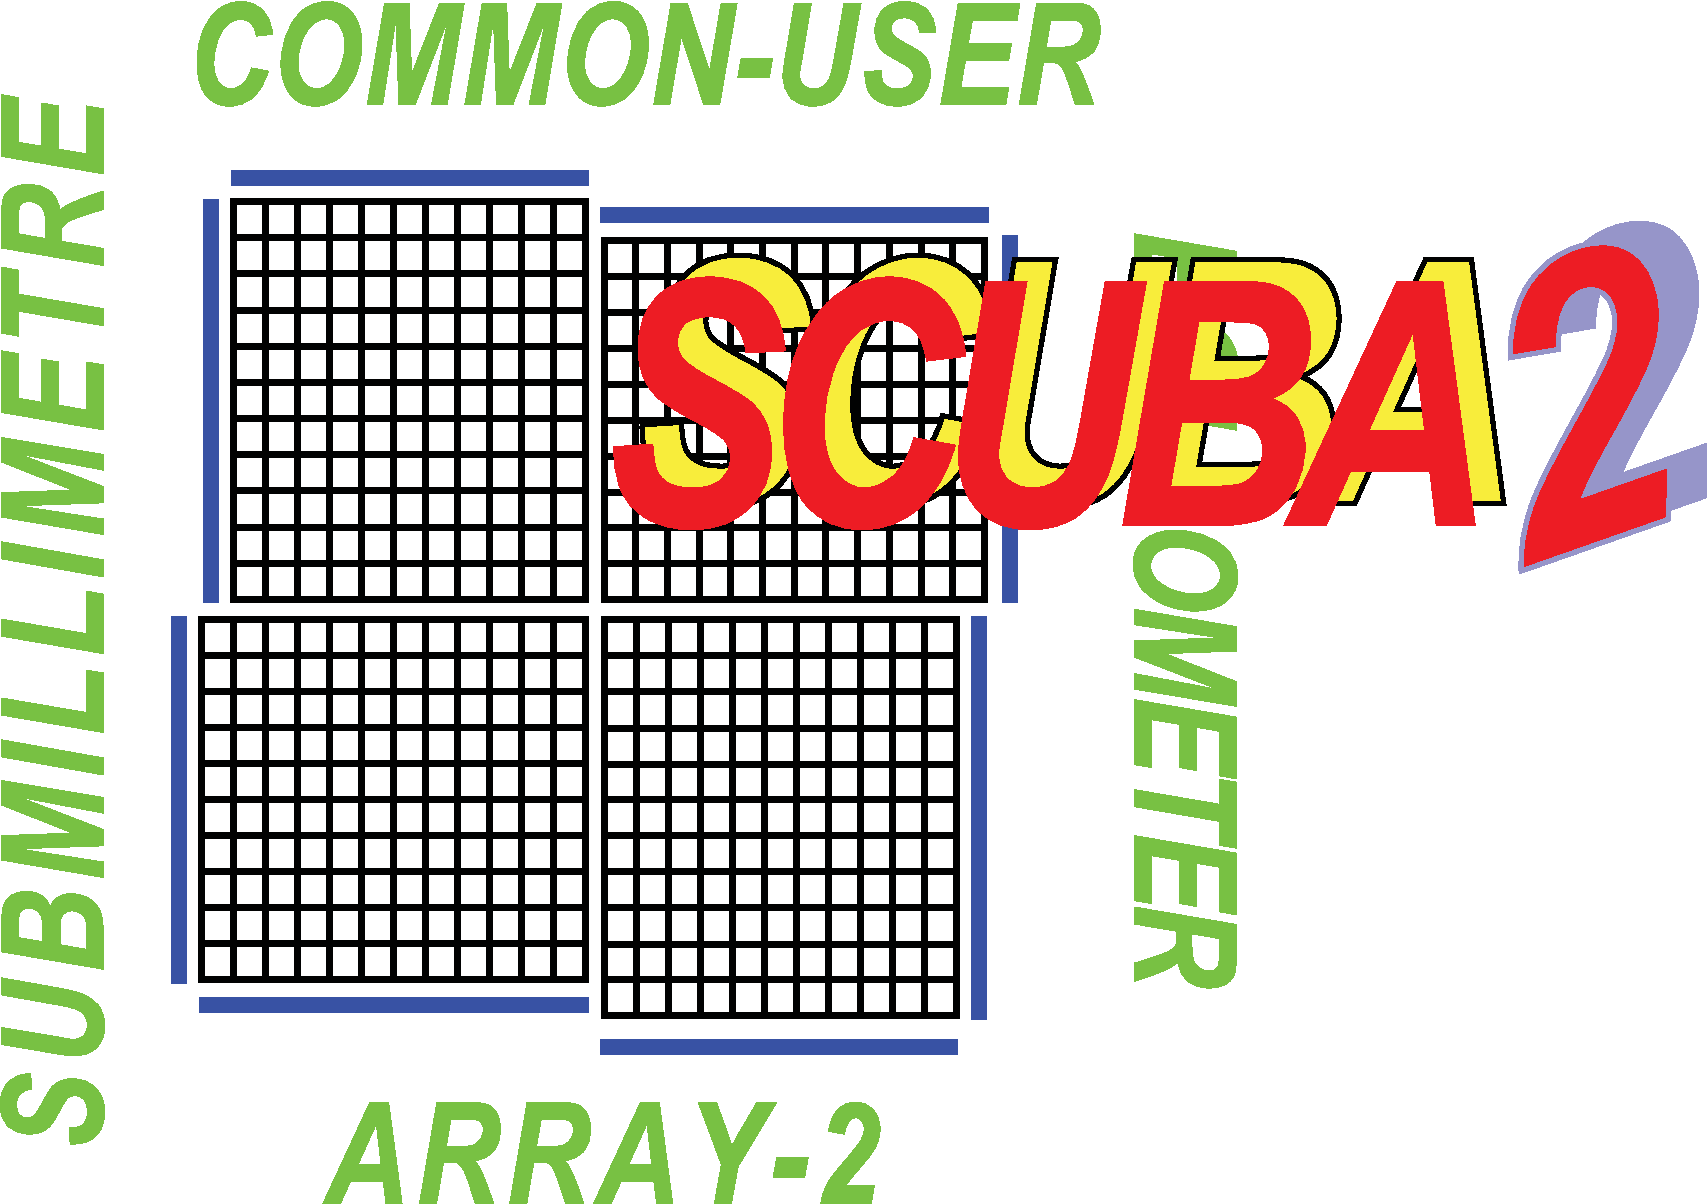
\includegraphics[scale=0.3]{sun264_logo}
\end{center}
% ? End of picture

% ? Heading for abstract if used.
   \vspace{10mm}
   \begin{center}
      {\Large\textbf{Abstract}}
   \end{center}
% ? End of heading for abstract.
\end{latexonly}

%  HTML documentation header.
%  ==========================
\begin{htmlonly}
   \xlabel{}
   \begin{rawhtml} <H1> \end{rawhtml}
      \stardoctitle\\
      \stardocversion\\
      \stardocmanual
   \begin{rawhtml} </H1> <HR> \end{rawhtml}

% ? Add picture here if required for the hypertext version.
%   e.g. \includegraphics[scale=0.7]{filename.ps}
\includegraphics[scale=0.7]{sun258_logo}
% ? End of picture

   \begin{rawhtml} <P> <I> \end{rawhtml}
   \stardoccategory\ \stardocnumber \\
   \stardocauthors \\
   \stardocdate
   \begin{rawhtml} </I> </P> <H3> \end{rawhtml}
      \htmladdnormallink{University of British Columbia}
                        {http://www.ubc.ca} \\
      \htmladdnormallink{Joint Astronomy Centre}
                        {http://www.jach.hawaii.edu}\\
      \htmladdnormallink{Science \& Technology Facilities Council}
                        {http://www.pparc.ac.uk} \\
   \begin{rawhtml} </H3> <H2> \end{rawhtml}
      \htmladdnormallink{Starlink Software Collection}{http://starlink.jach.hawaii.edu/}
   \begin{rawhtml} </H2> \end{rawhtml}
   \htmladdnormallink{\htmladdimg{source.gif} Retrieve hardcopy}
      {http://starlink.jach.hawaii.edu/cgi-bin/hcserver?\stardocsource}\\

%  HTML document table of contents.
%  ================================
%  Add table of contents header and a navigation button to return to this
%  point in the document (this should always go before the abstract \section).
  \label{stardoccontents}
  \begin{rawhtml}
    <HR>
    <H2>Contents</H2>
  \end{rawhtml}
  \htmladdtonavigation{\htmlref{\htmladdimg{contents_motif.gif}}
        {stardoccontents}}

% ? New section for abstract if used.
  \section{\xlabel{abstract}Abstract}
% ? End of new section for abstract
\end{htmlonly}

% -----------------------------------------------------------------------------
% ? Document Abstract. (if used)
%  ==================
\stardocabstract
% ? End of document abstract

% -----------------------------------------------------------------------------
% ? Latex Copyright Statement
%  =========================
\begin{latexonly}
\newpage
\vspace*{\fill}
\stardoccopyright
\end{latexonly}
% ? End of Latex copyright statement

% -----------------------------------------------------------------------------
% ? Latex document Table of Contents (if used).
%  ===========================================
  \newpage
  \begin{latexonly}
    \setlength{\parskip}{0mm}
    \tableofcontents
    \setlength{\parskip}{\medskipamount}
    \markboth{\stardocname}{\stardocname}
  \end{latexonly}
% ? End of Latex document table of contents
% -----------------------------------------------------------------------------

\cleardoublepage
\renewcommand{\thepage}{\arabic{page}}
\setcounter{page}{1}

% Main text

\section{\xlabel{introduction}Introduction\label{se:intro}}

The SCUBA-2 pipeline is a suite of recipes and primitives for the
\oracdr\ automated data processing software package. Additional
functionality for processing and analysis of reduced data is provided
through a number of \picard\ recipes. General documentation on \oracdr\
can be found in \oracsun.

The fundamental operation of the pipeline is to begin with raw data
and produce calibrated science images with no additional user
input. All decisions are based on metadata stored in the data files
combined with basic quality assessment of reduced data products.

\subsection{Document conventions}

In an attempt to make this document clearer to read, different fonts
are used for specific structures.

Observing modes are denoted by all upper case body text (e.g.\
FLATFIELD).

Starlink package names are shown in small caps (e.g.\ \SMURF);
individual task names are shown in sans-serif
(e.g.\ \makemap). \oracdr\ recipes and primitives are also shown in
sans-serif and are always upper case (e.g.\ \task{REDUCE\_SCAN}).

Content listings are shown in fixed-width type (sometimes called
`typewriter'). Extensions and components within NDF (\ndfref) data
files are shown in upper case fixed-width type (e.g.\
\ndfcomp{HISTORY}).

Text relating to filenames (including suffices for data products), key
presses or entries typed at the command line are also denoted by
fixed-width type (e.g.\ \texttt{\% smurf}), as are parameters for
tasks which are displayed in upper case (e.g.\ \aparam{METHOD}).

References to Starlink documents, i.e., Starlink User Notes (SUN),
Starlink General documents (SG) and Starlink Cookbooks (SC), are given
in the text using the document type and the corresponding number
(e.g.\ SUN/95). Non-Starlink documents are cited in the text and
listed in the bibliography.

File name suffices represent the text between the final underscore
character and the three-letter \verb+.sdf+ extension. For example, a
file named \verb+s4a20101020_00002_0001_cal.sdf+ has the suffix
\verb+_cal+.

\section{\xlabel{pipelines}SCUBA-2 Pipeline Variants\label{se:pipelines}}

There are three variants of the SCUBA-2 pipeline, two of which are
designed to run in real time at the JCMT. Most users will only need to
run the third form, the science pipeline.

\begin{itemize}
\item The quick-look (QL) pipeline is designed to process data and
  create images as quickly as possible, taking whatever short cuts are
  necessary to produce an image before the next data file is written
  to disk.

\item The summit pipeline runs in parallel with the QL pipeline
  (though on a different machine) and takes a more conservative
  approach. Processing is delayed until sufficient data exist to
  produce a higher quality image. An image is made when either a
  certain fraction of the observation is complete (the default is
  90\%), or the scan pattern has been completed once, whichever occurs
  first.

\item The science pipeline has access to all the data observed for a
  given project and adopts a best-possible reduction approach. Images
  are made for each complete observation which are combined to create
  the final image. (Note, however, that data from different nights
  will be processed separately and must be combined after the pipeline
  has finished.)
\end{itemize}

\subsection{Requirements for running the SCUBA-2 pipeline}

The SCUBA-2 pipeline requires a recent Starlink installation. The
Starlink environment should be initialized as usual before running
\oracdr. The latest version may be obtained here...

The software used to process raw data into images is called the
SubMillimetre User Reduction Facility (SMURF). Detailed documentation
on SMURF can be found in \SMURFsun, while \SMURFcook\ is a cookbook
that describes some of the background to SCUBA-2 data reduction.

The pipeline uses the following Starlink applications:

\begin{itemize}
\item \SMURF
\item \KAPPA
\item \FLUXES
\item \CCDPACK
\end{itemize}

The Starlink Perl installation (Starperl) must be used to run the
pipeline due to the module requirements, and \oracdr\ requires the use
of the TC-shell to work correctly.

\subsection{Important environment variables}

The pipeline uses a number of environment variables to determine where
data should be read from and written to. Some are set automatically
when the pipeline is initialized, but they can be overridden manually
and, with the \verb+-honour+ flag, may be left unchanged.

\begin{itemize}

\item \verb+$ORAC_DATA_ROOT+: root location for data. At the JCMT,
  this is \verb+/jcmtdata/raw/scuba2+. If not defined, the current
  directory is assumed.

\item \verb+$ORAC_DATA_IN+:

\item \verb+$ORAC_DATA_OUT+:

\item \verb+$MAKEMAP_CONFIG_DIR+:

\item \verb+$STARLINK_DIR+: location of the user's Starlink
  installation.


\end{itemize}


\section{\xlabel{runpipeline}Running the SCUBA-2 pipeline at the JCMT\label{se:runpipe}}

At the summit the pipeline is normally started by the telescope
support specialist (TSS) as normal user accounts do not have the
access privileges to write to the data output directories.

Each pipeline waits for new data to appear before processing, and
processes all data automatically choosing the correct recipe based on
the observation type (which may be modified by the particular pipeline
being run).

The QL pipeline is started with the following commands (substitute 850
for 450 for the short wave pipeline):

\begin{myquote}
\begin{verbatim}
% oracdr_scuba2_850_ql
% oracdr &
\end{verbatim}
\end{myquote}

The QL pipeline is fed data via DRAMA parameters and must be told the
names of the tasks to expect data from. The task names are
communicated through the \verb+ORAC_REMOTE_TASK+ environment
variable, and are usually of the form \verb+TASK@server+, e.g.,
\verb+SC2DA8D@sc2da8d+. The task name is in upper case; the machine
name serving the parameter in lower case.

The summit pipeline is started by:

\begin{myquote}
\begin{verbatim}
% oracdr_scuba2_850_summit
% oracdr -loop flag -skip &
\end{verbatim}
\end{myquote}

A user logged in on a regular account may monitor the pipeline
progress and have images displayed locally. To do this, run the
appropriate initialization script above to access either the QL or
Summit pipeline output and then run:

\begin{myquote}
\begin{verbatim}
% oracdr_scuba2_850_[summit|ql]
% oracdr_monitor &
\end{verbatim}
\end{myquote}

which will launch a clone of the \oracdr\ window so the user can follow
the output messages. The monitor will also launch its own display so
images and other diagnostic data can be viewed.


\section{\xlabel{offline}Offline processing of SCUBA-2 data\label{se:offline}}

\subsection{Running the Science pipeline}

\oracdr\ supports several ways to specify the data to process. A list
of all available command-line options may be obtained by running:

\begin{myquote}
\begin{verbatim}
% oracdr -h
\end{verbatim}
\end{myquote}

or

\begin{myquote}
\begin{verbatim}
% oracdr -man
\end{verbatim}
\end{myquote}

The options of interest for the purposes of this section are the
\verb+-files+, \verb+-loop+, \verb+-from+ and \verb+-list+.

If the data for your project have been downloaded from CADC and placed
in a single directory, the easiest procedure is to create a file
containing the full path to each of these raw files. The data can be
processed with the commands:

\begin{myquote}
\begin{verbatim}
% oracdr_scuba2_XXX
% oracdr -loop file -files <list_of_files.lis>
\end{verbatim}
\end{myquote}

where \verb+XXX+ is the wavelength (450 or 850). The initialization
command only needs to be run once.

Each observation is processed separately and the images combined to
form a single output image. If the list of files contains data from
different objects, the pipeline will treat each object separately and
create different output files accordingly.

The other options are applicable if running the pipeline at JAC or if
you have data arranged in the same as at the telescope. In this case
run \oracdr\ with the \texttt{-loop flag} option to indicate that the pipeline
should examine the contents of flag files (which end in \verb+.ok+). The flag
files contain the path to the files to be processed, and have a fixed
naming convention so the pipeline can recognize them.

\subsubsection{Processing Examples}

To process all files starting at observation 21 (skipping non-existent
files):

\begin{myquote}
\begin{verbatim}
% oracdr -loop flag -from 21 -skip
\end{verbatim}
\end{myquote}

To process the files from a list of observations (e.g. 21, 22, 28, 29 and
30):

\begin{myquote}
\begin{verbatim}
% oracdr -loop flag -list 21,22,28:30
\end{verbatim}
\end{myquote}

Note the use of a colon to specify a contiguous range of observation
numbers.

To process a set of data downloaded from the JCMT archive at CADC,
where the files to be processed have been listed in a text file called
\verb+data.lis+:

\begin{myquote}
\begin{verbatim}
% oracdr -loop file -files data.lis
\end{verbatim}
\end{myquote}

\subsection{Pipeline products}

The science data products from the pipeline have a suffix of
\verb+_reduced+. The files beginning with \verb+s+ are the products from
individual observations; the files beginning \verb+gs+ are the coadded
observations for a single object. The products from non-science
observations may have different suffices, and may be three-dimensional
cubes. See the documentation for individual recipes for further
details on those products.

In addition to the data files, the reduced products have PNG format
images 64, 256 and 1024 pixels on a side for easy viewing in an image
viewer or web browser.

\subsection{Calibration}

If no calibration observations are available, the pipeline will apply
standard flux conversion factors (FCFs) to calibrate the images in
mJy\,beam$^{-1}$. Currently these are 500000 mJy\,beam$^{-1}$ at
850\,$\mu$m and 400000 at 450\,$\mu$m.

\subsection{Customizing the map-making}

The pipeline uses the \SMURF\ dynamic iterative map-maker (\makemap)
to create maps from raw data. A detailed description of the map-maker
is given in \SMURFcook. The map-maker uses a configuration file to
control the data processing which may be modified by users with
advanced knowledge of the map maker. The SCUBA-2 pipeline may be given
the name of an alternative or customized configuration file via the
recipe parameter capability of \oracdr. A number of pre-defined
configuration files exist in the directory
\verb+$STARLINK_DIR/share/smurf+. Once a suitable configuration file
has been created, add its name to a recipe parameter file as follows:
\begin{myquote}
\begin{verbatim}
[REDUCE_SCAN]
MAKEMAP_CONFIG = myconfigfilename.lis
\end{verbatim}
\end{myquote}
and add \verb+-recpars recipe_params.lis>+ to the command line when
running the pipeline, where \verb+recipe_params.lis+ is the name of
recipe parameter file. The file must exist in the current working
directory or one of the directories defined by the environment
variables \verb+$ORAC_DATA_OUT+ or \verb+$MAKEMAP_CONFIG_DIR+. Each
directory is search in turn and the first match is used.

\section{\xlabel{details}Detailed description of the SCUBA-2 pipeline\label{se:details}}

\subsection{The QuickLook (QL) Pipeline}

Each new file on disk is processed in turn using the iterative map
maker with a configuration file optimized for short observations. If
the source is a known calibrator, then an FCF is derived. The data are
calibrated in mJy\,beam$^{-1}$ using default FCFs. This image is
displayed using \GAIA, showing in window 1, and then combined with the
current coadd image. The noise is determined for the coadd image and
stored in a log file. The coadd image is displayed in another
\GAIA\ window (2), and its error component (noise) in another (3). Any
temporary files created during this processing are deleted, keeping
only files with a suffix \verb+_reduced+.

\subsection{The Summit Pipeline}

As each file is picked up by the pipeline, it checks to see if the
scan pattern has been completed at least once since the beginning of
the observation (or since the last image was made) or if the
percentage completion parameter exceeds 90\%. If either of these
criteria are met, a new image is created using all the data which has
not previously been processed. If not, the raw data are flatfielded.

Thereafter, the summit pipeline follows the same procedure as the QL
until the final step with one important exception. The images for a
given source continue to be coadded. If a new image was not created
during the latest pass through the recipe then all flatfielded data
files needed to create a map are left on disk (suffix
\verb+_ff+). However, these files will be deleted once a new image is
made.

\subsection{The Science pipeline}

The science pipeline examines all the data files given to it and works
out which files are related and should be processed together. Each
observation is still processed separately to produce an image, which
is calibrated in mJy\,beam$^{-1}$. All the images for a given source are
combined into a single coadd using variance weighting. If the source
is a known calibrator then the images are checked for offsets and
shifted if necessary to align with the standard position.

Finally at the end of processing, all temporary files are deleted: the
only data files left on disk will have the suffix \verb+_reduced+.

Recipes exist for a number of different target types which contain
different processing steps, relevant to each particular target
type. These are bright or faint compact (such as planets, T Tauri
stars or extragalactic blank fields respectively) and extended (such
as Galactic star-forming regions). Examples of these steps include
applying a matched-filter to enchance point-source detectability, or

Furthermore it is anticipated that the JCMT Legacy Surveys will have
optimized processing recipes.

\section{\xlabel{nonscience}Processing of non-science data\label{se:nonsci}}

This section contains detailed information on how the SCUBA-2 pipeline
processes non-science observations and can be ignored by users only
interested in processing science data. Each of the observation types
are discussed in turn with relevant details on how they are processed
by the different forms of the pipeline.

\subsection{FLATFIELD}

Flatfield data may be taken in a standalone flatfield observation, but
they are also taken as part of science observing, where a fast-ramp
flatfield measurement is made at the beginning and end of the
observation.

Standalone flatfield observations are processed with the
\task{REDUCE\_FLATFIELD} recipe. A flatfield solution is derived for
each subarray present in each observation and written to an NDF file
with the suffix \verb+_flat+. The pipeline reports the number of good
bolometers and statistics of the responsivities, as well as how they
have changed relative to the existing flatfield solution (the one
present in the raw data files).

The new solution is also shown and compared with the previous one
graphically. Figure \ref{fig:flatfield} is an example of the display
for one subarray. The results for each subarray are displayed in a
separate window. The responsivities for the new and existing solutions
are shown as images side-by-side on the same scale. In addition a
percentage-change image is shown below (scaled between $\pm$5\,\% or
10\,\% at 850/450\,$\mu$m respectively), as well as histograms of the
new and existing responsities (again on the same scale).

\begin{figure}[ht]
\centering
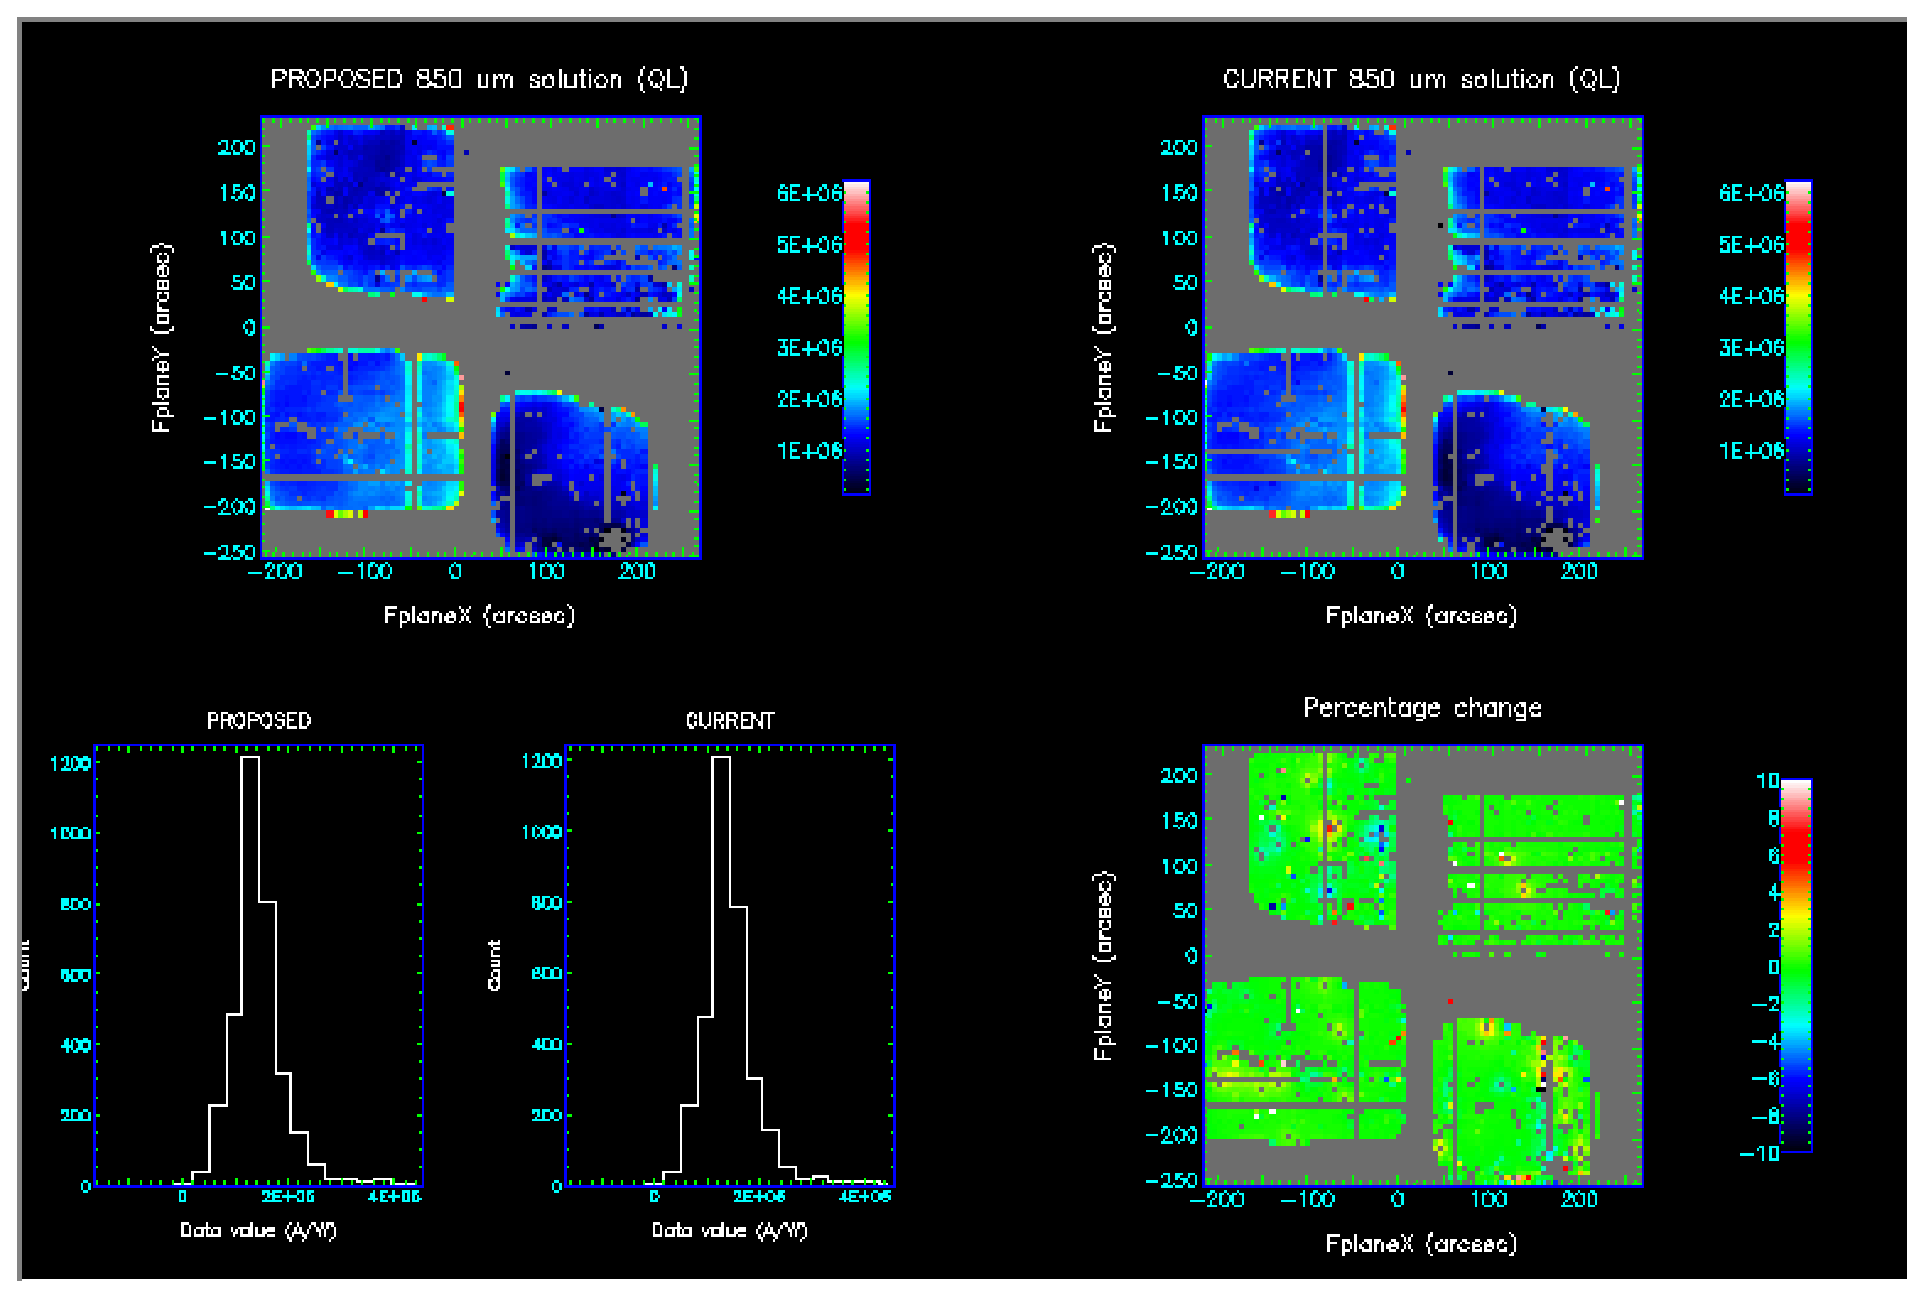
\includegraphics[width=\textwidth]{sun264_flatfield.eps}
\caption{Example display from a FLATFIELD observation. The top left
  panel is the responsivity map for this observation, the top right
  panel is the current responsivity solution in use for
  comparison. The bottom left panels are responsivity histograms for
  this observation and the current solution. The bottom right panel
  shows the percentage change in the responsivities between this
  observation and the current solution in use, scaled between $\pm10$
  per cent.\label{fig:flatfield}}
\end{figure}

Once complete, the pipeline writes a flag file in
\verb+$ORAC_DATA_OUT+ for the current observation containing the name
of each successful flatfield solution. The flag file is a hidden file
with the name \verb+.sYYYYMMDD_MMMMM.ok+ where \verb+YYYYMMDD+ is the
UT date and \verb+MMMMM+ is the zero-padded observation number. This
file is used by the telescope control system (TCS) at the JCMT to
identify the new flatfields to use in subsequent observations.

\subsubsection{Fast-ramps}

The fast-ramp flatfields taken as part of on-sky observing are
included with the science data and processed as part of map-making,
but may be processed separately using the \task{REDUCE\_FASTFLAT}
recipe to assess how much the responsivities change during an
observation. The results are calculated and displayed as above, but in
this case the second fast-ramp flatfield is compared with the first,
and not with the internal flatfield solution.

\subsection{NOISE}

Noise gets noisy...

\subsection{POINTING}

Pointing observations consist of making a map of a point source, and
are processed with the \task{REDUCE\_POINTING} recipe. The recipe
processes the data with the iterative map-maker, crops the image to
75\,arcsec on a side and removes any residual large-scale background
signal with \CUPID\ \task{findback}. If the source is a known
calibrator, the pipeline derives an FCF.

Once generated, the pipeline writes the name of the processed image
into a flag file (as for FLATFIELD observations above). The flag file
is read by the telescope POINTING\_FOCUS task which analyzes the named
image to calculate the pointing offsets applied to the pointing model.

The pipeline makes its own estimate of the pointing offsets in two
ways by applying a point-source filter (matched filter) to enhance the
signal-to-noise ratio in the image followed by fitting a 2-D profile
to the source and calculating the centroid position. Both results are
written to a log file called \verb+log.pointing+.

The pipeline displays the image used to derive the pointing offsets in
a \GAIA\ window. The recipe also calculates the beam size and writes the
result to a log file called \verb+log.beam+.

The map-maker uses the config file \verb+dimmconfig_pointing.lis+,
except for very short pointing observations (defined as $<15$\,s)
which use \verb+dimmconfig_veryshort_planet.lis+ for planets and
\verb+dimmconfig_bright_compact_veryshort.lis+ for all other sources.

The QL pipeline uses the \task{REDUCE\_POINTING\_QL} recipe, which
contains different logic for dealing with DREAM and STARE data but is
functionally identical to the main \task{REDUCE\_POINTING} recipe for
SCAN data.

\subsection{FOCUS}

Focus observations are processed with the \task{REDUCE\_FOCUS}
recipe. A focus observation consists of a series of maps made of a
point source with the secondary mirror (SMU) at various
positions. Only one axis is varied at a time.

In the QL pipeline, the maps are made as the data are taken and
collated once the observation has ended. (In practice, due to the fact
that the QL pipeline cannot rely on the \verb+OBSEND+ FITS header, an
observation is considered to have ended once an image exists at each
of the SMU positions: the number of SMU positions is retrieved from
the FITS header.) The non-QL pipeline processes each SMU setting in
turn.

Once all the maps exist, the pipeline creates a cube with the third
axis given by the SMU position. The images are registered to the same
pixel coordinates before adding to the cube so that they align
correctly.

The pipeline writes a flag file (as above) which contains the name of
the data cube. The flag file is read by the telescope POINTING\_FOCUS
task which analyzes the cube to calculate the best SMU position. The
pipeline makes its own estimate of the best-fit SMU position by
fitting a parabola to the peak fluxes derived from 2-D fits (provided
at least three fluxes could be derived) and writes that number to a
log file called \verb+log.focus+.

The images at each focus position are displayed in sequence in a
single Kapview window (see Figure \ref{fig:focus}).

\begin{figure}[th]
\centering
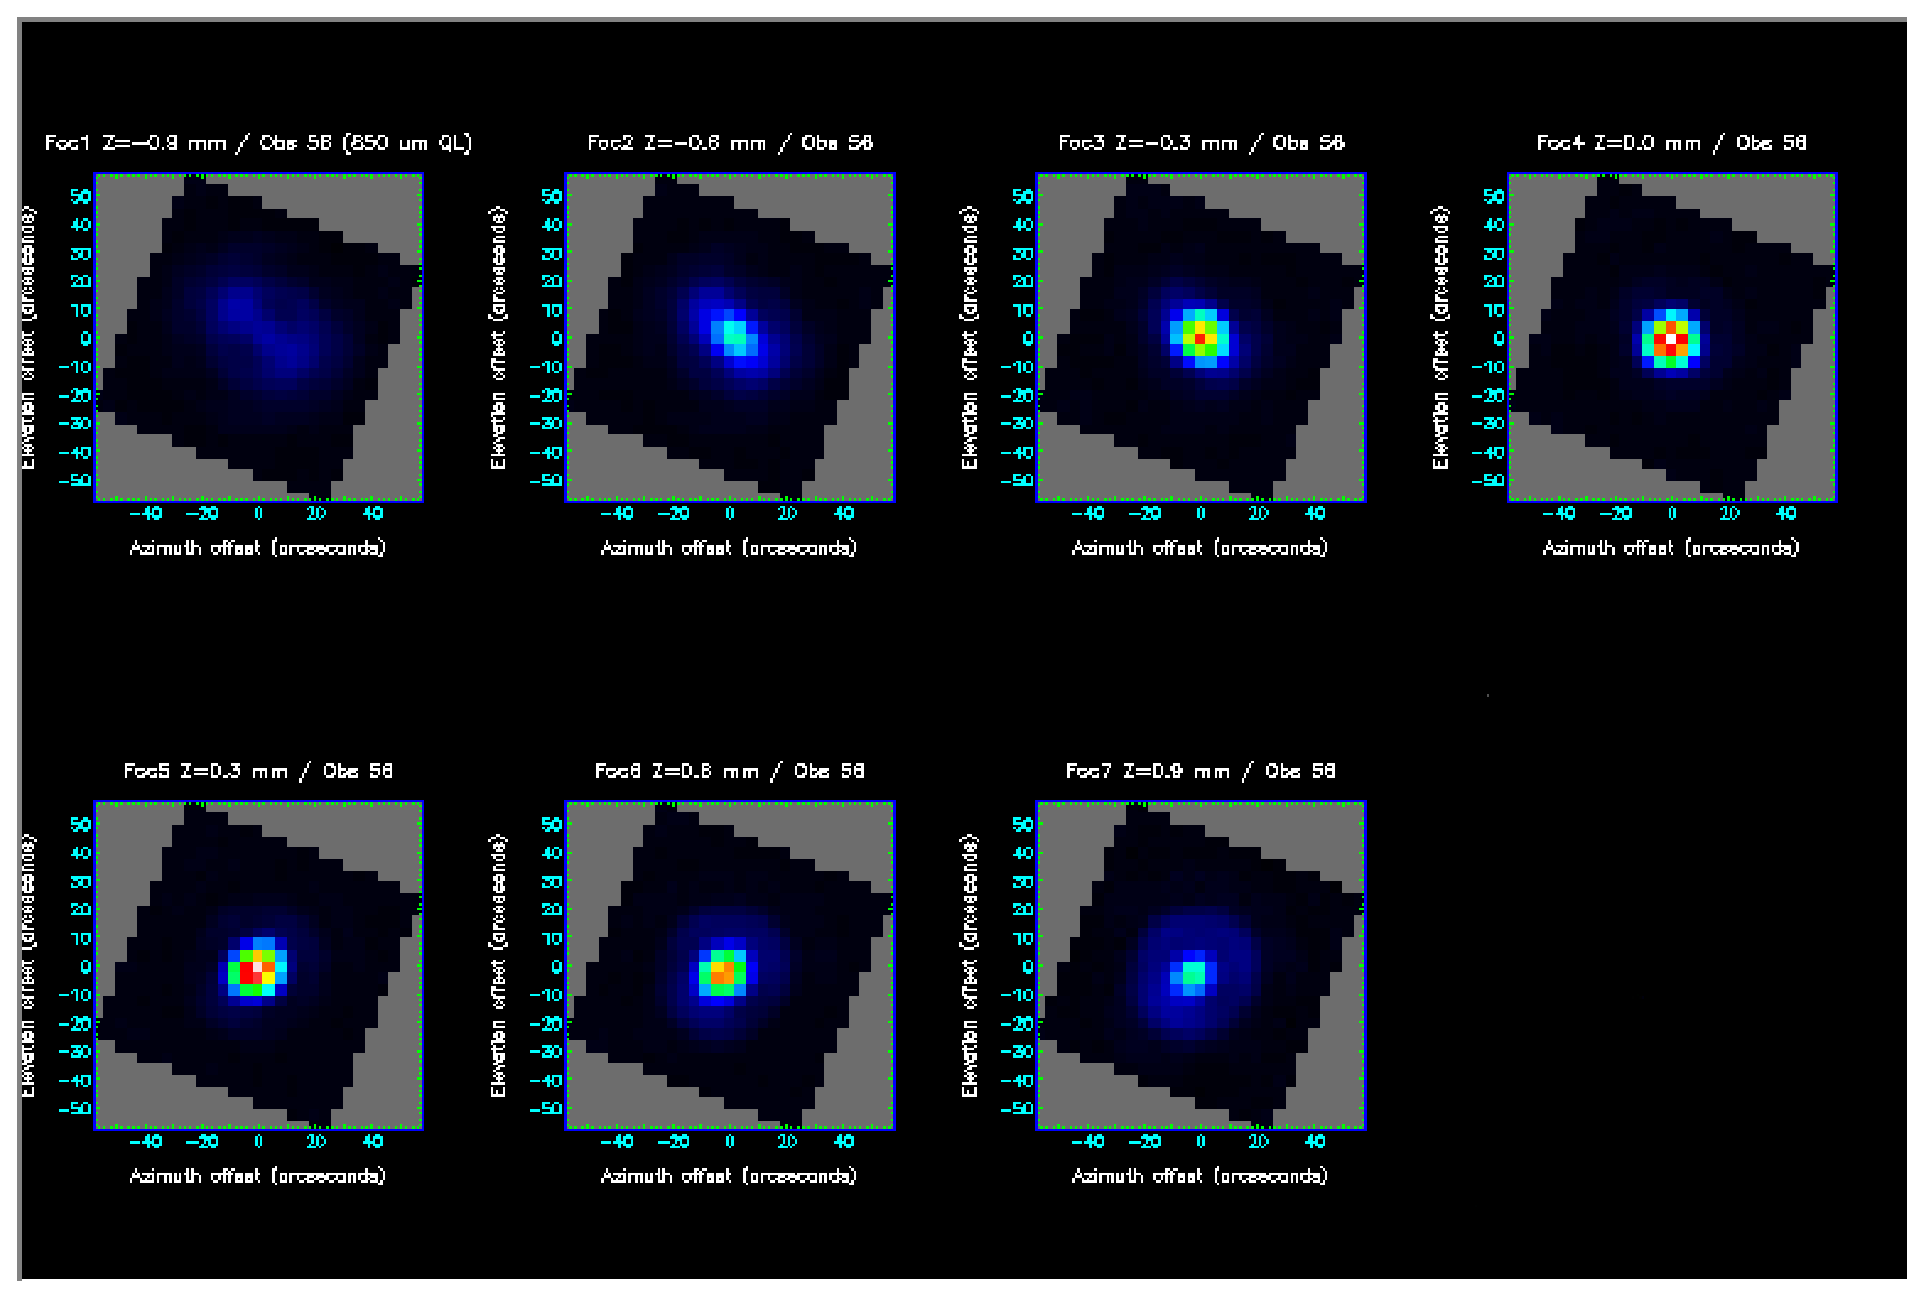
\includegraphics[width=\textwidth]{sun264_focus.eps}
\caption{Example display from a FOCUS observation showing a reduced
  image for each of seven SMU positions. The SMU position (and axis)
  is given in the title for each image. The images are displayed with
  axes of arcsecond offsets.\label{fig:focus}}
\end{figure}

The map-maker uses either the \verb+dimmconfig_veryshort_planet.lis+
for planets and \\ \verb+dimmconfig_bright_compact_veryshort.lis+ for
all other sources.

The same recipe is used for all forms of the pipeline. The output cube
has the suffix \verb+_foc+.

\subsection{SKYDIP}

A SKYDIP observation is a series of NOISE-SKY observations at
differing airmass. Currently there is no pipeline recipe to process
these data, other than as a NOISE observation.


\section{\xlabel{engineering}Engineering Data\label{se:eng}}

Recipes also exist for processing engineering data, usually taken with
the shutter closed and the telescope stationary. Historically, the
real-time sequencer (RTS) was not involved in such measurements which
prevented the pipeline from processing these data due to missing FITS
headers and other essential metadata.

A decision was made in September 2010 that the pipeline be used to
process and analyze data taken in engineering mode, and a simulated
RTS is used to generate metadata. Support for engineering data is
currently quite rudimentary with only a single recipe available.

\subsection{NEP}

Measurements of the noise-equivalent power (NEP) are processed with
the \task{ENG\_NEP} recipe. The `observation' consists of a series of
NOISE measurements at different pixel heater and detector bias
values. The recipe is designed to run offline, after the observation
has finished.

The NEP is calculated for each subarray at each setting. These
per-bolometer NEP images are combined to form a 4-d hypercube with
axes bolometer row, bolometer column, heater setting and bias setting
for each subarray. These hypercubes are named
\verb+sXXYYYYMMDD_MMMMM_nep.sdf+ where \verb+sXX+ is the subarray
label (e.g.\ \verb+s8a+).

From these data, the effective and RMS NEP is calculated at each
heater and bias setting, stored as a 2-d image with the heater and
bias values as the X- and Y axes. These images have suffices of
\verb+_effnep+ and \verb+_rmsnep+ respectively.

A number of log files are also written. The first is called
\verb+log.bolonoise+ which contains the noise properties for each
heater and bias setting and all subarrays. Log files for the `mapping
speed' parameter for each subarray are written separately. The mapping
speed is given by $N_{\rm bol} / NEP_{\rm RMS}^2$ and is calculated
for the best $N_{\rm bol}$ bolometers between 300 and 1000 in steps of
100 bolometers.

The recipe does not display any data.

\section{\xlabel{dataproducts}Data products (output files)\label{se:dataprod}}

data array
variance/error
exp\_time

\section{\xlabel{picard}Analysis of processed data\label{picard}}

A variety of simple \picard\ recipes exist to perform post-processing
analysis.

SCUBA-2 specific \picard\ recipes all begin with the prefix
\verb+SCUBA2_+; recipes specific to processing JCMT data contain
\verb+JCMT+. The current list may be obtained by listing the contents
of the directory \verb+${ORAC_DIR}/recipes/PICARD+ or by visiting the
\picard\ home
page,\\ \htmladdnormallink{\texttt{http://www.oracdr.org/oracdr/PICARD}}{http://www.oracdr.org/oracdr/PICARD}
where each recipe is fully documented.

The recommended approach for a few common tasks is detailed below.

\subsection{Coadding/mosaicking multiple images}

Although the pipeline will mosaic observations of the same target from
the same night, it is clearly desirable to combine data from multiple
nights. Alternatively, the user may wish to exert some additional
control over the mosaicking parameters.

The \task{MOSAIC\_JCMT\_IMAGES} recipe deals with processed JCMT data
(including ACSIS data cubes) and takes into account the
instrument-specific NDF components such as the exposure time
(\verb+EXP_TIME+ -- see \S\ \ref{se:dataprod} above). The choice of
coadding task is left to the user and may be either
\CCDPACK\ \task{makemos} or \KAPPA\ \task{wcsmosaic} (the default). If
using \task{makemos}, images are first aligned using
\KAPPA\ \task{wcsalign}. By default, the images (and additional NDF
components) are combined using a nearest-neighbour scheme but this may
be overridden by specifying the relevant parameter for
\task{wcsmosaic} or \task{wcsalign}.

For images which contain a bright source, there is also the option to
register the images to a common centre (see \S\ \ref{se:reg}
below). If chosen, the user must provide the coordinates (equatorial
in sexagesimal format, i.e.\ \verb+HH:MM:SS.S, DD:MM:SS.S+) of that
source, unless it is a known calibrator (in which case the WCS
reference position will be used instead). Note that choosing this
option will modify the WCS of the input files. If this is not desired,
the user should register the images separately (\S\ \ref{se:reg}).

The output mosaic takes its name from the last input file in the list
and has the suffix \verb+_mos+.

\subsection{Registering images to a common centre\label{se:reg}}

Random pointing offsets and drifts between observations on a given
night (and over different nights) mean that the final mosaic of a
point source will not be optimal, and any faint surrounding structure
may be masked entirely.

The recipe \task{SCUBA2\_REGISTER\_IMAGES} is specific to SCUBA-2
data.  The approach is to find the position of a given source in each
image and apply a shift to the WCS so that the peak fitted positions
are coincident for each image.

Several recipe parameters are required, namely the coordinates of the
reference position. Currently only equatorial coordinates are
supported and must be written in sexagesimal format. The registered
images have the suffix \verb+_reg+.

As with the mosaicking recipe, this recipe knows about and takes care
of applying the same shift to the \verb+EXP_TIME+ and \verb+WEIGHTS+
components, so the combined results are accurate.

\end{document}

